\begin{wrapfigure}{r}{0.5\textwidth}%
\centering%
\vspace{-1cm}
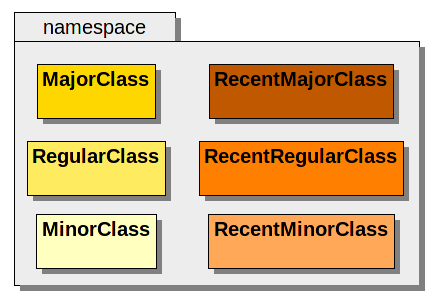
\includegraphics[scale=.33]{../classdiagrams/uml-legend.png}%
\caption{Color conventions in UML diagrams.}%
\label{fig:uml-legend}%
\end{wrapfigure}%

\section{Introduction}

This chapter present the design of \sofa{}, as well as its recent evolutions.
It also includes discussions justifying some of the decision that are behind this design.

The conventions used in UML class diagrams is presented in Fig~\ref{fig:uml-legend}.

\vspace{.8cm}

\section{Core}

\subsection{Object Model (\textcode{sofa::core::objectmodel})}

\begin{figure}[h]
\centering
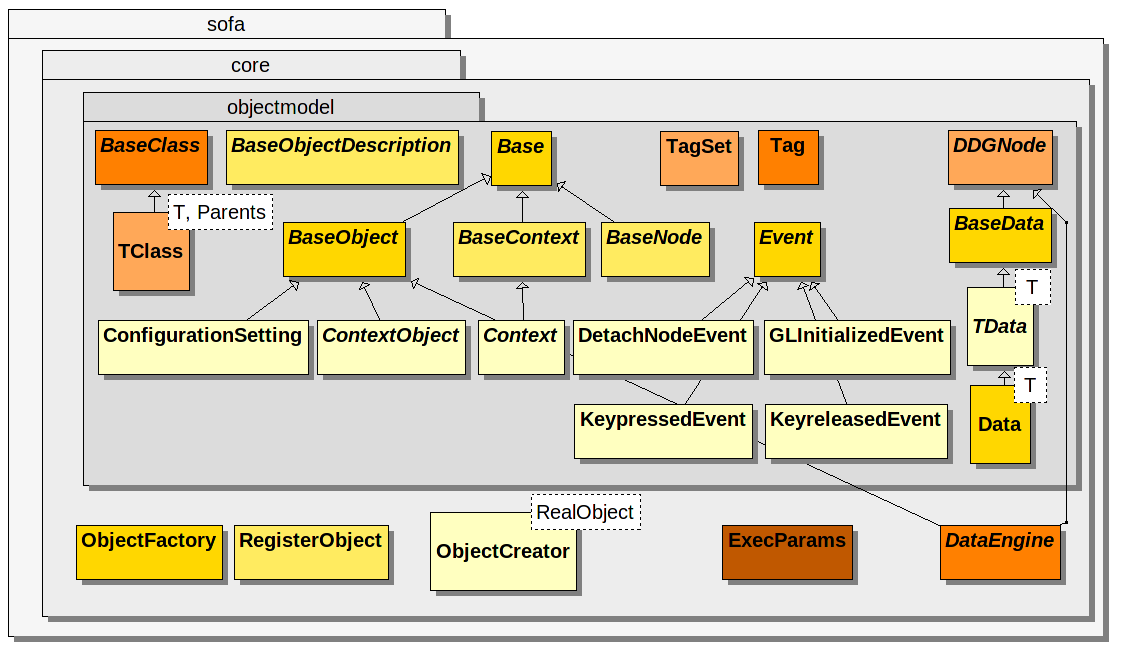
\includegraphics[scale=.33]{../classdiagrams/sofacore-objectmodel.png}
\caption{Classes of the \textcode{sofa::core::objectmodel} namespace.}
\label{fig:uml-sofa-core-objectmodel}
\end{figure}

\subsubsection{Changes compared to the 1.0~beta~4 version}

\paragraph{New class description system.}
It is based on the \textcode{BaseClass} and \textcode{TClass} classes, and requires to add the \textcode{SOFA\_CLASS} macro in the declaration of all classes deriving from Base.
The benefits are that it is now possible to follow the full hierarchy of classes from the final components, instead of having just a fixed set of categories.
This macro is also necessary in classes with a templated parent class to be able to use methods and member variables defined in \textcode{Base} such as \textcode{initData} or \textcode{sout}. This removed all the previously redundant direct heritage to \textcode{BaseObject} that was previously required.

\paragraph{Objects and node tagging (\textcode{Tag} and \textcode{TagSet}).}
The goal of the introduction of tags is to provide one of the pieces necessary to support non-mechanical states (electrical potentials, constrast agent concentrations) as well as cleaner non-geometrical mechanical states (fluid dynamics, reduced-coordinate articulations).
For example, in a simulation involving blood in deformable vessels, we would use two tags to distinguish the different states : mechanical, fluid.
These tags will be used to easily work with only a subset of the components, so that the mechanical solver works on positions and forcefields but don't interferes with blood flow and pressure, and inversely for the fluid solver.
See \url{http://wiki.sofa-framework.org/tdev/wiki/Notes/ProposalGenericStates} for more information.
We decided on using there tags instead of extending the class hierarchy as was done before with the \textcode{State} and \textcode{MechanicalState} classes.
A hierarchy is fine when we have only one feature that we want to differentiate on (such as base vs mechanical vs electrical), but when we add other criteria (lagrangian geometry vs eulerian vs reduced generalized coordinates, velocity vs vorticity, independent vs mapped DOFs) it is no longer manageable as specialized classes.
A secondary use of these tags is to replace existing subsets mechanisms within CollisionModels (r2441) and Constraints (r3121).
The design is based on the following elements.
Tags are added to BaseObject, as a list of string (internally converted to a list of unique ids for faster processing).
All visitors now filter the objects they process based on their list of tags.
All solvers by default copy their own list of tags to the visitors they execute, so that they only affect the objects with the same tags as they have (TODO: this is currently broken). 

\paragraph{Dependencies between Data (\textcode{DDGNode} and \textcode{DataEngine}).}
The goal is to be able to specify simple links between datas or through computation engines.

\paragraph{\textit{Copy-on-Write} (CoW) mechanism (\textcode{DataContainer}).}
The goal is to reduce copies of datas when using engines and/or multi-threading.

\paragraph{Support for asynchronous multi-threading (\textcode{ExecParams}).}

~

\pagebreak

\subsection{Physical Behavior (\textcode{sofa::core::behavior})}
\begin{figure}[h]
\centering
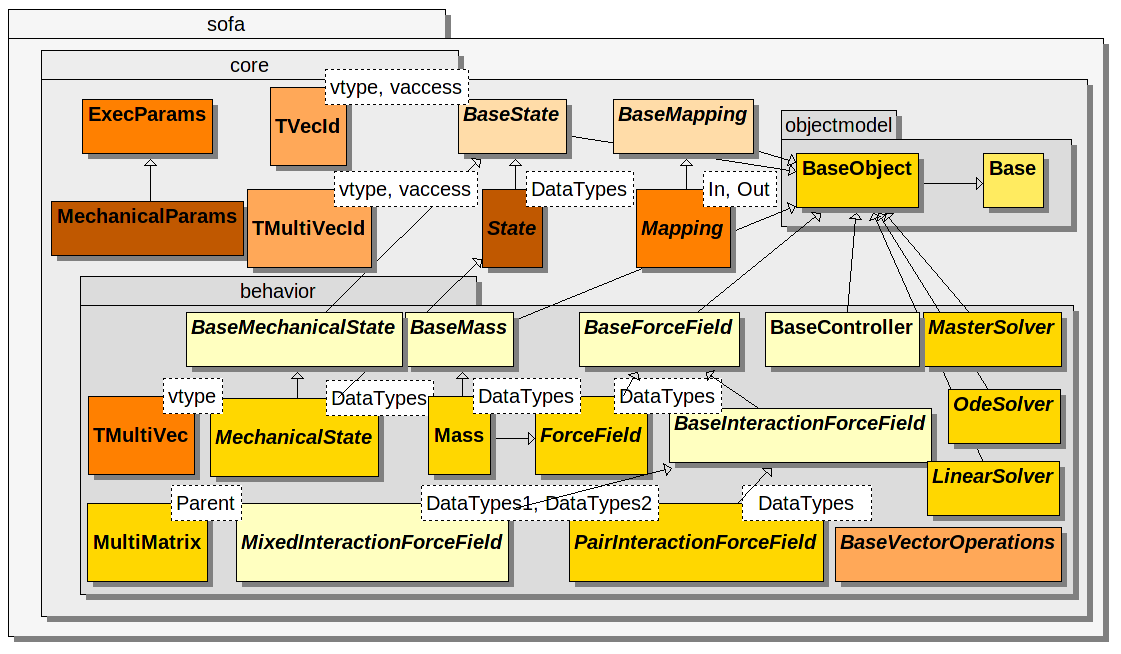
\includegraphics[scale=.33]{../classdiagrams/sofacore-behavior.png}
\caption{Classes of the \textcode{sofa::core::behavior} namespace.}
\label{fig:uml-sofa-core-behavior}
\end{figure}

\subsubsection{Changes compared to the 1.0~beta~4 version}



%% \section{Framework}

%% \subsection{UML Diagrams}

%% \begin{figure}[h]
%% \centering
%% 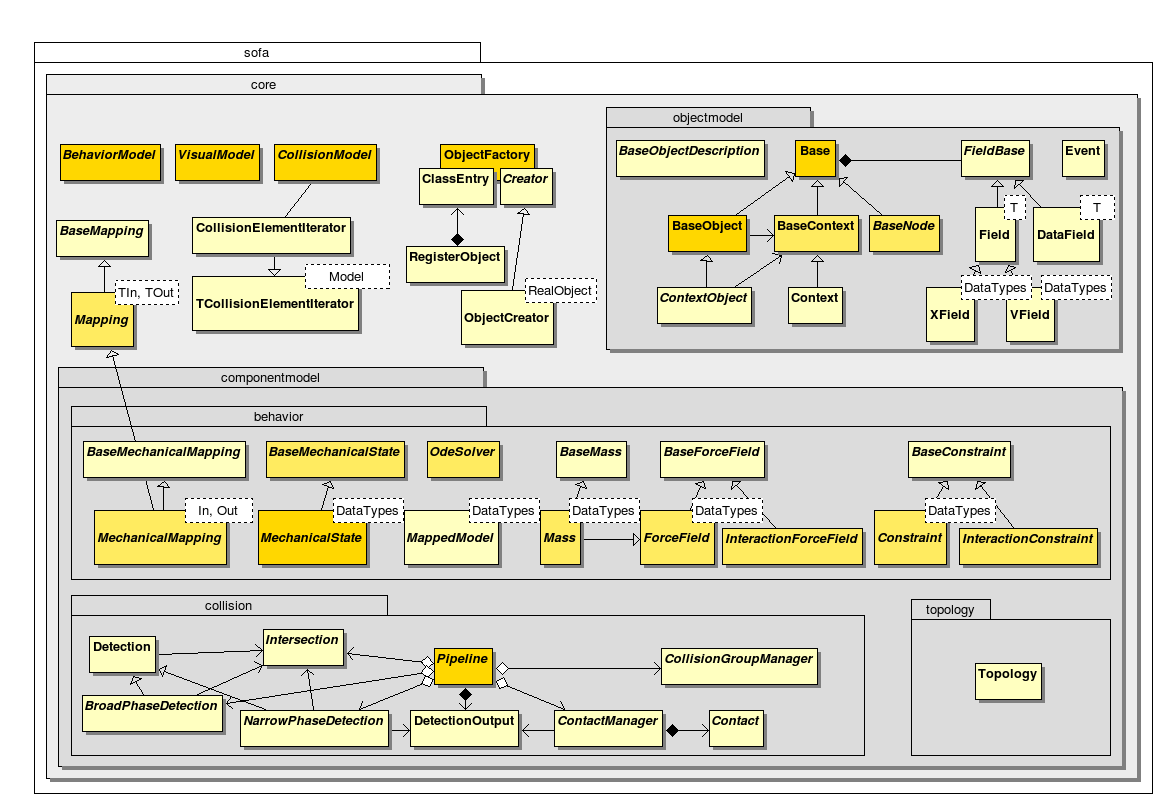
\includegraphics[width=\linewidth]{uml-sofa-core.png}
%% \caption{Classes of the sofa::core namespace.}
%% \label{fig:uml-sofa-core}
%% \end{figure}
